% 本文档编写于 2022 年 9 月 13 日,使用 TeXLive 2022 编译通过
% 请使用不低于 2021 版的 TeXLive (在苹果系统上可以是 MacTeX) 编译此文档
% 其它编译器不保证编译效果的正确性,不要使用早已过时并且存在许多 bug 的 CTeX 套装

%==============================%
%   清华大学求真书院讲义模板   %
%   清华大学求真书院版权所有   %
%==============================%

\documentclass[UTF8,oneside,11pt]{book}
                               % UTF8 指定文件编码
                               % oneside 指定书籍为单开页 (防止多余的空白页出现)
\usepackage[a4paper,margin=1in]{geometry}
                               % 设置纸张大小为 A4,页边距为1英寸

\usepackage{amsmath}           % AMS 的主包
\usepackage{amssymb}           % AMS 符号包,会自动加载 amsfonts
\usepackage{latexsym}          % 几个额外的特殊符号,包括 \Box
\usepackage{mathrsfs}          % \mathscr 字体样式
\usepackage{eucal}             % 更改 \mathcal 的字体样式
\usepackage{amsthm}            % AMS 的定理环境
\usepackage{mathtools}         % 一些额外的数学环境功能,包括 \dfrac
\usepackage{stmaryrd}          % 更更多的特殊符号
\usepackage{esint}             % 更多积分符号
\usepackage{extarrows}         % 提供在箭头上下写字的命令
\usepackage{enumerate}         % 带序号列表环境
\usepackage{xcolor}            % 让 latex 支持花里胡哨的颜色的包
\usepackage{graphicx}          % 插入各种类型图片支持
\usepackage{tikz}              % tikz 绘图环境
\usepackage{tikz-3dplot}       % 一个简单的 tikz 3d 绘图宏包
\usepackage{tikz-cd}           % 基于 tikz 的交换图表绘制工具
\usepackage[all,cmtip]{xy}     % 交换图表绘制工具,命令为 \xymatrix
\usepackage{pgfplots}          % 高级绘图包,基于 tikz,包括 2d 和 3d 绘图
\pgfplotsset{compat=newest}    % 设置 pgfplots 兼容性选项,以使用新功能
\usepackage{subcaption}        % 可以交叉引用的图表并排环境
\usepackage[ocgcolorlinks,linkcolor=blue]{hyperref}
                               % 更 fancy (如带颜色,可以点击等等) 的引用
\usepackage{cleveref}          % 更“聪明”的引用,使用此宏包,在引用一个公式/定理等时
                               % 请使用 \cref 而非 \ref
\usepackage[hyperref=true,backend=biber,style=alphabetic,backref=true,url=false]{biblatex}
                               % 使用 biblatex 管理参考文献,后端采用 biber,取代
                               % 古老的 natbib + bibtex,使用方法自行上网查阅
                               % 如果需要用 natbib,请自行注释掉这一行然后正常使用
\usepackage{tcolorbox}         % 绘制彩色文本框的宏包
\tcbuselibrary{most}           % 加载 tcolorbox 的库
\usepackage{bm}                % 为所有数学字体添加粗体,命令 \bm{abcd}
\usepackage{slashed}           % 在符号上添加反划线,命令 \slashed

%==============================%
%     请在这里添加其它宏包     %
%------------------------------%
% \usepackage{physics}         % 提供了方便地打出 d/dx 等符号的命令
% \usepackage{float}           % 我用来防止插图浮动 <- 你不需要它
\usepackage{tensor}            % 张量指标



%==============================%

%==============================%
%    私货,定义了一些小命令    %
%------------------------------%
\DeclareMathOperator{\sign}{sign}
\DeclareMathOperator{\dom}{dom}
\DeclareMathOperator{\ran}{ran}
\DeclareMathOperator{\ord}{ord}
\DeclareMathOperator{\rank}{rank}
\DeclareMathOperator{\Span}{span}
\DeclareMathOperator{\img}{Im}
\DeclareMathOperator{\dd}{d\!}
\newcommand{\card}{\texttt{\#}}
\newcommand{\ie}{\emph{i.e.}}
\newcommand{\st}{\emph{s.t.}}
\newcommand{\eps}{\varepsilon}
\newcommand{\vphi}{\varphi}
\newcommand{\vthe}{\vartheta}
\newcommand{\II}{I\!I}
\renewcommand{\emptyset}{\varnothing}


%==============================%

%==============================%
%         定理环境设置         %
%------------------------------%
\theoremstyle{plain}\newtheorem{thm}{Theorem}
\theoremstyle{definition}\newtheorem{defn}[thm]{Definition}
\theoremstyle{plain}\newtheorem{axiom}[thm]{Axiom}
\theoremstyle{plain}\newtheorem{coro}[thm]{Corollary}
\theoremstyle{plain}\newtheorem{lemma}[thm]{Lemma}
\theoremstyle{plain}\newtheorem{prop}[thm]{Proposition}
\theoremstyle{plain}\newtheorem{conj}[thm]{Conjecture}
\theoremstyle{plain}\newtheorem{prob}[thm]{Problem}
\theoremstyle{plain}\newtheorem{const}[thm]{Construction}
\theoremstyle{remark}\newtheorem{notation}[thm]{Notation}
\theoremstyle{definition}\newtheorem*{ques}{Question}
\theoremstyle{definition}\newtheorem*{ans}{Answer}
\theoremstyle{definition}\newtheorem*{goal}{Goal}
\theoremstyle{plain}\newtheorem*{app}{Application}
\theoremstyle{plain}\newtheorem*{exam}{Example}
\theoremstyle{plain}\newtheorem*{exer}{Exercise}
\theoremstyle{remark}\newtheorem*{remark}{Remark}
\theoremstyle{remark}\newtheorem*{note}{\small{Note}}
\numberwithin{equation}{section}
\numberwithin{thm}{section}
%==============================%

%==============================%
%    定义标题图片和背景图片    %
%------------------------------%
\usepackage{fancyhdr}
\pagestyle{fancy}
\fancypagestyle{plain}{
    \renewcommand{\headrulewidth}{0pt}
    \fancyhead{}
    \chead{
\includegraphics[width=0.4\linewidth]{picture/qiuzhen.png}} 
}
\renewcommand{\headrulewidth}{0pt}
\addtolength{\headheight}{0.025\paperheight}
\addtolength{\topmargin}{-0.025\paperheight}
\fancyhead{}
\chead{
\includegraphics[width=0.4\linewidth]{picture/qiuzhen.png}} 
%------------------------------%
% \usepackage{eso-pic}
\DeclareHookRule{shipout/background}{title/opac}{before}{pgfrcs}
\AddToHook{shipout/background}[title/opac]{
    \begin{tikzpicture}[remember picture,overlay]
        \centering
        \node [opacity=0.1] at (current page.center) {
            
\includegraphics[height=0.2\paperheight]{picture/redqiuzhen.png}
        };
    \end{tikzpicture}
}
%==============================%

%==============================%
%  添加参考文献库 (.bib 文件)  %
%  例 \addbibresource{XX.bib}  %
%------------------------------%

\addbibresource{}

%==============================%

%==============================%
% 定义封面样式,请将 XX 替换为 %
% 具体的课程名和人名           %
%------------------------------%
\title{
    \huge{Differential Geometry~~Lecture Notes}
    \vspace{0.4\paperheight}
}
\author{
    \Large{Instructor: Zhang Yingying}\\
    \Large{Notes Taker: Xue Haotian, Yan Guangxi}
    \vspace{0.1\paperheight}
}
\date{
    \Large{Qiuzhen College, Tsinghua University}\\
    \Large{2022 Fall}
}                                         
%==============================%

\begin{document}
\maketitle
\frontmatter
\tableofcontents
\newpage

%==============================%
%           正文内容           %
%------------------------------%

\mainmatter{}

\chapter*{\centering Preface}
\addcontentsline{toc}{chapter}{Preface}
\setlength{\headheight}{33.24858pt}
\section*{Textbook Reference}
\begin{enumerate}[(1)]
    \item Do Carmo: Differential Geometry of Curves and Surfaces.
    \item Sebasti\'an Montiel, Antorio Ros: Curves and Surfaces.
    \item \textit{Chinese Title, add later}
\end{enumerate}
\section*{Course Introduction}
The Goal of this course is to study the ``differential geometry of curves and surfaces''.

\noindent
$\bullet$ \textbf{Geometry}: How is a geometric object curved / How to measure the curvedness of a geometric object? 
\begin{example}
     In the illustration below, (1) differs by ``topology''. In (2), they are topologically the same, while the lower curve is ``more curved'' than the upper curve.
\end{example}

\begin{center}
    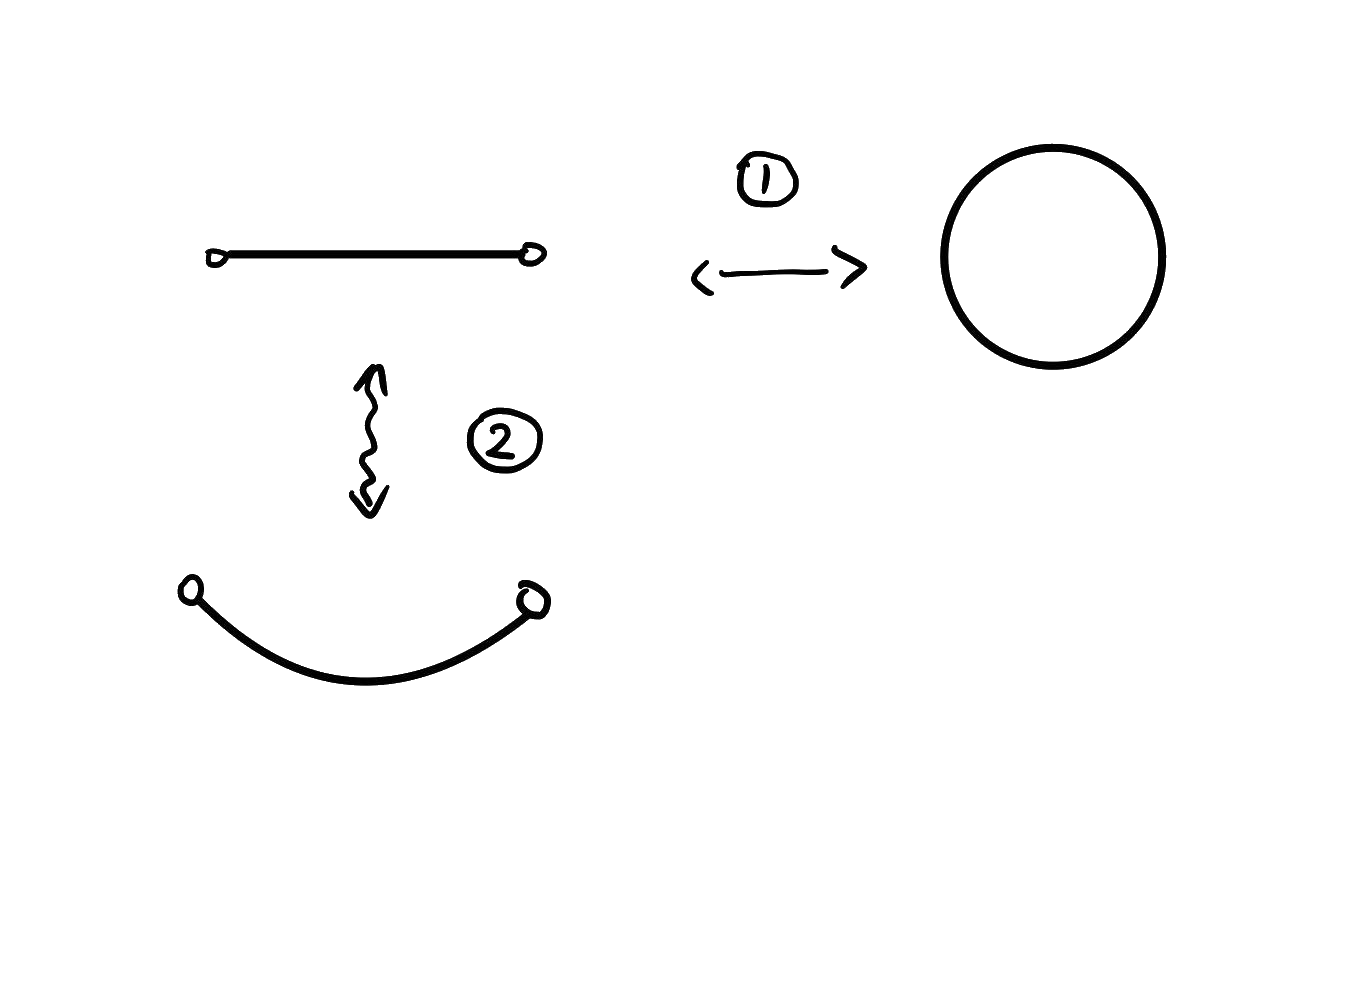
\includegraphics[scale=0.3]{picture/preface/preface_example1.png}
\end{center}

\begin{example}
    (3) differs by ``topology'', but in (4) $\mathbb{S}^2(1)$ is more curve than $\mathbb{S}^2(2)$, even topologically they are the same.(either homeomorphically or diffeomorhically).
\end{example}

\begin{center}
    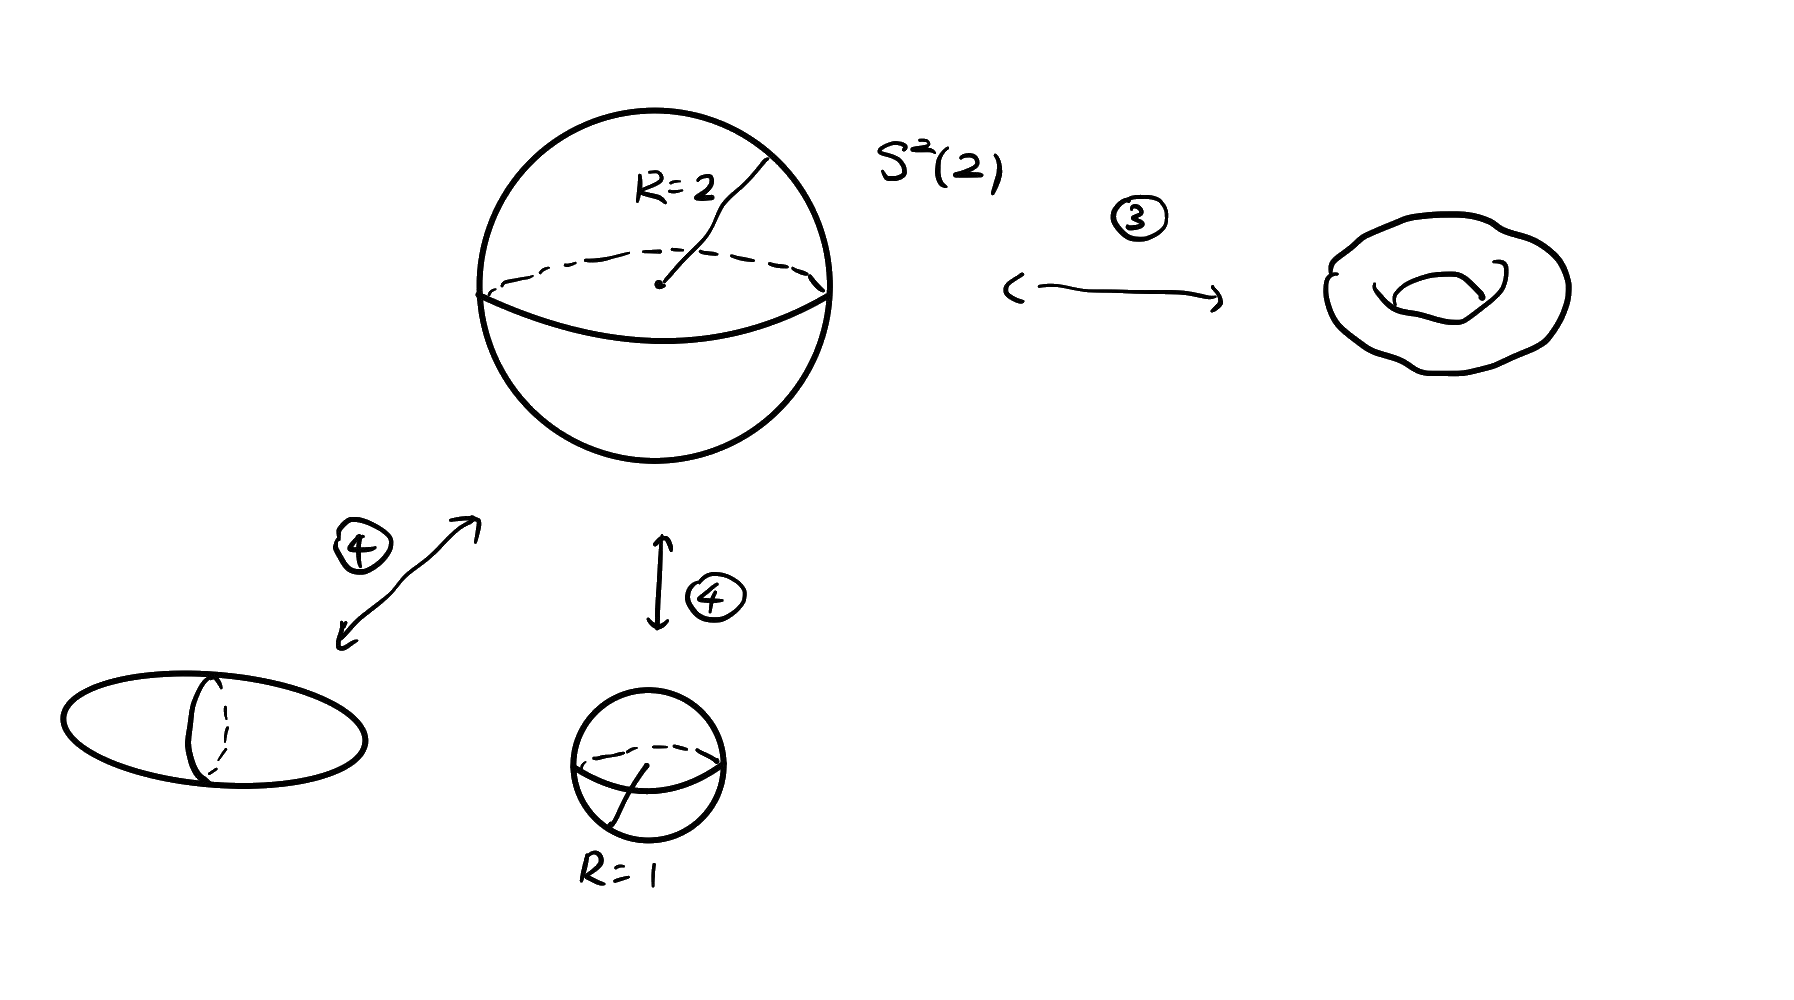
\includegraphics[scale=0.2]{picture/preface/preface_example2.png}
\end{center}

The ``Curved property'' also affects geometric quantities, like length, area, volume, angle between the curves, etc.

\textbf{Local Geometry}: How does a ``curved '' space look like in a neighborhood of a point?
 
\textbf{Global Geometry}: If we know how a ``curved space'' is look like at each point, can we observe how such space looks like globally? This is usually related to topological problems.

$\bullet$ \textbf{Differential}: In this course, by ``smoothness'' we mean the geometric objects we'll study are ``nice'' enough so we can apply ``calculus'' tools to study them.

\textbf{Main tool}: Calculus! We'll see how powerful calculus is in this course, especially, like the maximal principle, integration by parts(stoke's theorem), Taylor's expansion, implicit function theory, etc.

\begin{center}
    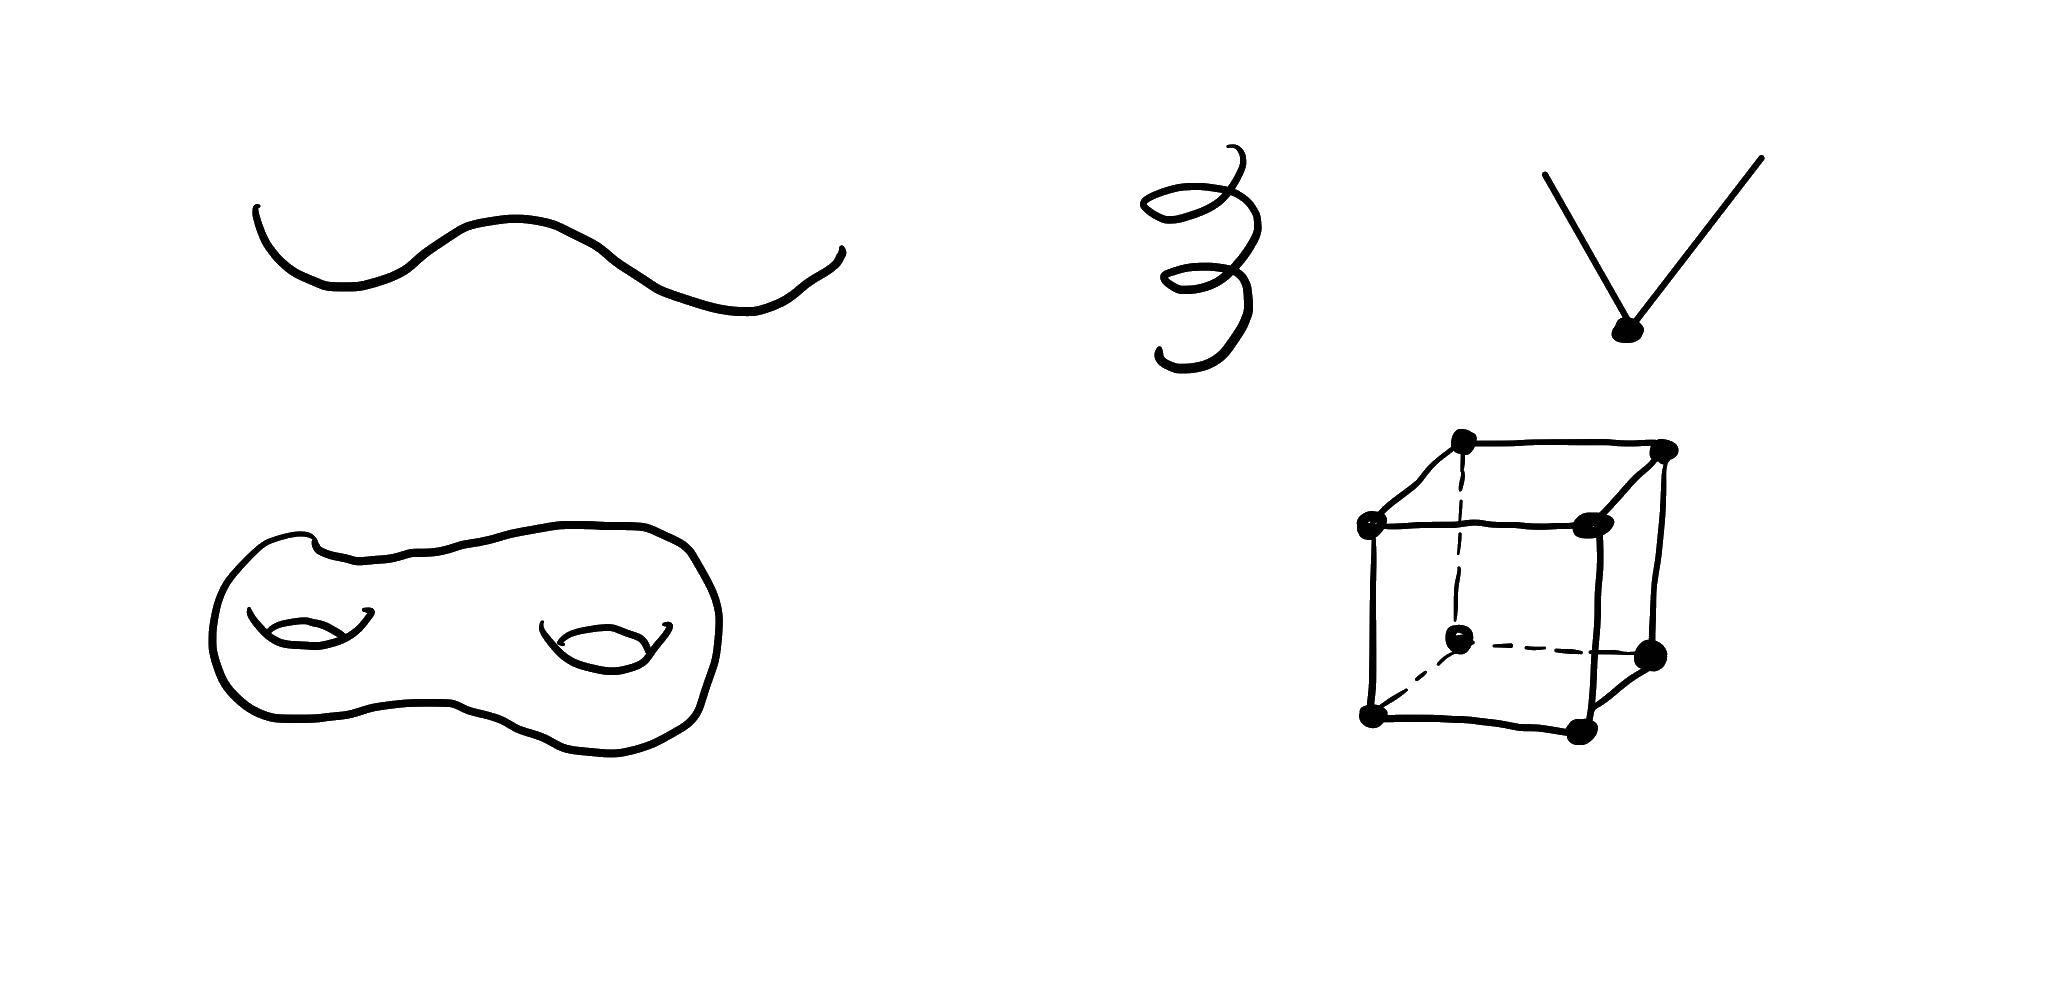
\includegraphics[scale=0.2]{picture/preface/preface_example3.png}
\end{center}

Queastion: How to tell the ``smoothness''?(Need to find good parametrization)Finding a good ``gauge''(that is ``coordinate'') to work with is also an important question in geometry.

$\bullet$Curves: 1-d geometric object.

Surfaces: 2-d geometric object.
\begin{remark}
    In this course, we only focus on curves and surfaces in $\mathbb{R}^3$.However, as a training on preparing for later geometry course, I suggest you also try to think about the ambiant space is $\mathbb{S}^3$ or $\mathbb{H}^3$.

\end{remark}
$\bullet$\textbf{Intrinsic geometry}: Study the geometric object without considering the ambient space. This begins from the Gauss's elegant theorem and was developed by Riemann.
\begin{example}
    Consider the unit sphere $\mathbb{S}^2$

    Extrinsic geometry: view it as $x^2+y^2+z^2=1$ in $\mathbb{R}^3$.

    Intrinsic geometry: $(\theta,\varphi)$ or $(\varphi,\theta)$ are ``essential'' coordinates on $\mathbb{S}^2$. \[
        \dd s^2=\dd \varphi^2+(\sin\varphi)^2 \dd\theta^2
    \]

    (Caution: $(\theta,\varphi)$ is outer normal, while $(\varphi,\theta)$ is inner normal.)
\end{example}
$\bullet$ Useful / Common techniques:
\begin{enumerate}[1)]
    \item Comparison: compare the studied geometric object with ``model space''. It's very important to study examples in geometry. As a suggestion you are expected to spend time to play with $\mathbb{S}^2$.For example: How is $\mathbb{S}^2$ curved? What's the shortest line in $\mathbb{S}^2$? How many symmetries are there on $\mathbb{S}^2$? Can you add ``extra structure'' on$\mathbb{S}^2$ to make it a complex object? Is this ``extra structure'' ``rigid''?What/s the ``moment map'' on $\mathbb{S}^2$? Does there exist a ``holomorphic'' map from $\mathbb{S}^2$ to a torus, or a surface of arbitrary genus? 
 
    If we consider an ``Energy minimizing map'' from $\mathbb{S}^2$ to $\mathbb{S}^2$, what can we say about such map?(It is  holomorphic/antiholomorphic.)
 
    After you have learned Riemann Geometry, you'll see an energy minimizing map from $\mathbb{S}^2$ to a Riemannian manifold must be an angle-preserving map(conformal map).
 
    What kinds of 2-d geometric space could be $\mathbb{S}^2$ ?(this is a global geometry problem.)(\ie\ what kinds of geometric conditions can characterize $\mathbb{S}^2$ ?)
    \item To study higher dimensional objects,it's also important to understand lower dimensional objects, and it's also important to understand lower dimensional objects contained in the studied objects.
    \item Study ``functions'' (more generally sections, including functions, vector fields, differential forms, etc.) on a given geometric object.
\end{enumerate}
\begin{example}
    On a closed surface ( $\mathbb{S}^2$,$\mathbb{T}^2$,$\Sigma_g$)(compact without boundary) there is no non-constant harmonic function.(i.e. $\Delta u=0$)(Analysis will get involved.)
\end{example}
We usually care about those functions related to geometry, such as distance functions, curvature-related functions, etc.
\begin{example}[More trivial than the last one]
    Consider $f''(x)=0$, what can you say of the solution of it when $x$ lies on a line and when $x$ lies on a circle?
\end{example}


\chapter{Differential Geometry of Curves}
\section{Linear algebra convention and its geometric explanation}
\begin{itemize}
    \item We use ``ROW VECTOR'' in this course, \ie\
    \[v\in \mathbb{R}^n, v=(v_1,v_2,\cdots,v_n)\]
    \item let $e_1=(1,0,\cdots,0),\cdots,e_n=(0,\cdots,1)$ be the standard basis, then 
    \[v=\sum_{i=1}^nv^i e_i=
    \begin{bmatrix}
        v^1& v^2& \cdots & v^n
    \end{bmatrix}
    \begin{bmatrix}
        e_1\\
        e_2\\
        \vdots\\
        e_n
    \end{bmatrix}
    \]
    \item $\varphi\colon \mathbb{R}^n\to \mathbb{R}^n$ (non-degenerate) linear map
    \[v\mapsto \varphi(v)=v\cdot A.\]
    This corresponds to the right action of $GL(n,\mathbb{R})$ on $\mathbb{R}^n$.
    \[\Rightarrow \varphi(e_i)=e_j \cdot A=\sum_{i=1}^n A\indices{_j^i}e_i\text{ (taking the j-th row of }A\text{)}\]
    
    \[A\indices{_j^i}\begin{cases}
        \text{upper index: column index}\\
        \text{lower index: row index}
    \end{cases}\]
    \[\Rightarrow \varphi\begin{bmatrix}
        e_1\\
        e_2\\
        \vdots\\
        e_n
    \end{bmatrix}=\begin{bmatrix}
       \varphi( e_1)\\
        \varphi (e_2)\\
        \vdots\\
        \varphi(e_n)
    \end{bmatrix}=\begin{bmatrix}
        e_1\cdot A\\
        e_2\cdot A\\
        \vdots\\
        e_n\cdot A
    \end{bmatrix}=
    A \begin{bmatrix}
        e_1\\
        e_2\\
        \vdots\\
        e_n
    \end{bmatrix}\]
\end{itemize}
\begin{remark}[Important!]
    In row vector convention, a non-degenerate linear map corresponds to the right action of $GL(n,\mathbb{R})$ on $\mathbb{R}^n$. But this induces left action of $GL(n,\mathbb{R})$ on the orthonormal basis (frame) $\{e_1,e_2,\ldots,e_n\}$. This phenomenon provides an important example in differential geometry, which will be explained later in the theory of principle bundle.(\ie\ let $G$ be a lie group, $G\curvearrowright M$ being a right action, where $M$ is a differentiable manifold, then this right action induces a left action of $G$ on the frame bundle of $M$.)
 \end{remark}
 
 
 Let $\{\tilde{e}_1,\ldots,\tilde{e}_n\}$ be another basis of $\mathbb{R}^n$. Let $f$ be the corresponding linear map, \ie\
 \[f\begin{bmatrix}
    e_1\\
    e_2\\
    \vdots\\
    e_n
\end{bmatrix}=\begin{bmatrix}
    \tilde{e}_1\\
    \tilde{e}_2\\
    \vdots\\
    \tilde{e}_n
\end{bmatrix}=B \cdot \begin{bmatrix}
    e_1\\
    e_2\\
    \vdots\\
    e_n
\end{bmatrix}\]
\[\Rightarrow \tilde{e}_k=\sum_{j=1}^n B\indices{_k^j}e_j\]
We compare the matrix of $\varphi$ in terms of $\left\{\tilde{e}_1 \cdots \tilde{e}_n\right\}$
\[
    \varphi\left[\begin{array}{c}\tilde{e}_1 \\ \vdots \\ \tilde{e}_n\end{array}\right]=\varphi\left[B\left[\begin{array}{c}\tilde{e}_1 \\ \vdots \\ e_n\end{array}\right]\right]=B \cdot \varphi\left[\begin{array}{c}e_1 \\ \vdots \\ e_n\end{array}\right]\text{(linearity of }\varphi\text{)}
\]
\[
    =B A\left[\begin{array}{c}
    e_1 \\
    \vdots \\
    e_n
    \end{array}\right]=B A B^{-1}\left[\begin{array}{c}
    \tilde{e}_1 \\
    \vdots \\
    e_n
    \end{array}\right]
\]
Note in this case.
\[
(\varphi \circ f)\left[\begin{array}{c}
e_1 \\
\vdots \\
e_n
\end{array}\right]=B A\left[\begin{array}{c}
e_1 \\
\vdots \\
e_n
\end{array}\right]
\]
In terms of entries,
\begin{align*}
    \varphi(\tilde{e}_k) &=\varphi(\sum_{j=1}^n B\indices{_k^j} e_j)=\sum_{j=1}^n B\indices{_k^j} \varphi(e_j) \quad \text { (linearity) } \\
    &=\sum_{i, j=1}^n B\indices{_k^j} A\indices{_j^i} e_i=\sum_{i,j,p=1}^n B\indices{_k^j} A\indices{_j^i}(B^{-1})\indices{_i^p} \widetilde{e}_p
\end{align*}
\begin{remark}
    This computation tells that the row vector convention yields to the fact that $GL(n,\mathbb{R})$ acting on itself from the right when we consider the action of $GL(n, \mathbb{R})$ on $\mathbb{R}^n$.
    In modern Geometry, it's more common to use column vector as convention. This row vector convention was adopted by S.S. Chern and also Do Cormo's book.
\end{remark}
\section{Parametrized Curves}
\begin{definition}
    Let $I=(a,b)$, if $\alpha\colon I\to \mathbb{R}^3$ is a $C^\infty$ map,
    \[t \mapsto (x(t),y(t),z(t))\]
    then $\alpha(t)$ is a parametrized differentiable curve in $\mathbb{R}^3$. The image of $\alpha$ is called the trace of the curve. 
\end{definition}
\begin{remark}
    \hfill
    \begin{enumerate}[1)]
        \item $a,b$ could be finite number or infinity.
        \item Same curve may have different parametrizations.
        \item The parametrization automatically gives the direction of the motion on the curve.
        \item ``Differentiable'' just means $\alpha(t)$ is a $C^\infty$ \textbf{map}, it does not say the (trace of) curve can not have singularities.
    \end{enumerate}
\end{remark}
\begin{example}
    \hfill
    \begin{enumerate}[(1)]
        \item $\alpha(t)=(t,|t|)$ is not a differentiable curve.
        \begin{center}
            \begin{tikzpicture}
                \draw[domain=-2:0,smooth,variable=\t,black]
                plot (\t,{-\t});
                \draw[domain=0:2,smooth,variable=\t,black]
                plot (\t,\t);    
                \draw (0,0) node{$\bullet$};
                \draw[->] (-2,0) -- (2,0) node[right] {$x$};
                \draw[->] (0,-0.5) -- (0,2.5) node[above] {$y$};
            \end{tikzpicture}
        \end{center}
        \item $\alpha=(t^3,t^2)$ is a differentiable curve. It can be also given by a equation $y^3=x^2$, which is a cuspidal cubic curve.
        \begin{center}
            \begin{tikzpicture}
                \draw[domain=-1.5:1.5,smooth,variable=\t,black]
                plot ({\t^3},{\t*\t});
                \draw (0,0) node{$\bullet$};
                \draw[->] (-2,0) -- (2,0) node[right] {$x$};
                \draw[->] (0,-0.5) -- (0,2.5) node[above] {$y$};
            \end{tikzpicture}
        \end{center}
        \item $\alpha(t)=(t^2-1,t^3-t)$. This parametrization appers in the ``blow-up'' process of $y^2=x^3+x^2$. Here ``blow-up'' is introducing tangents to seperate points.
        \begin{center}
            \begin{tikzpicture}
                \draw[domain=-1.5:1.5,smooth,variable=\t,black]
                plot ({\t*\t-1},{\t^3-\t});
                \draw (0,0) node{$\bullet$};
                \draw[->] (-2,0) -- (2,0) node[right] {$x$};
                \draw[->] (0,-2.5) -- (0,2.5) node[above] {$y$};
            \end{tikzpicture}
        \end{center}
    \end{enumerate}
\end{example}
\begin{remark}
    (2) and (3) above may be the first examples you'll see in an algebraic geometry course.
\end{remark}
\noindent
\textbf{Question}: At the origin, what can you obsefve on (2) and (3)?

\noindent
\textbf{Answer}:
    (2) $\alpha'(0)=0$.
    (3) $\alpha$ is not one to one, but $\alpha'(0)\neq 0$.

\noindent 
\textbf{Question}: Define a differentiable curve in $\mathbb{R}^3$ and $\mathbb{S}^n$.
\begin{remark}
    Among above differentiable parametrizations, (2) and (3) are differentiable curves. However, if we take $\beta(t)=(t,t^{\frac{2}{3}})$, this also parametrizes (2), but it's not a differentiable curve!
\end{remark}
\begin{definition}
    Let $\alpha(t)\colon I\to \mathbb{R}^3$ be a parametrized differentiable curve, then at $t_0\in I$.
    \[ \alpha'(t_0)=(x'(t_0),y'(t_0),z'(t_0))\]
    is the velocity of $\alpha(t)$ at $t_0$.
    \begin{enumerate}[(1)]
        \item If $\alpha'(t_0)\neq 0$, we call $\alpha(t_0)$ a regular point.
        \item If $\alpha'(t_0) = 0$, we call $\alpha(t_0)$ a singular point.
        \item If for all $t\in I$, $\alpha'(t)\neq 0$, we call $\alpha(t)$ a regular curve.
    \end{enumerate}
\end{definition}
\noindent
\textbf{Question}: What can you say about $C^\infty$ parametrization for a regular curve?
\begin{quotation}
Regular curve $\Longleftrightarrow $ at each point, there is a unique tangent line.
\end{quotation}
\begin{example}
$\alpha(t)=(t^3,t^2)$ is not a regular curve. (Since $\alpha'(0)=0$)
\begin{center}
    \begin{tikzpicture}
        \draw[domain=-1.5:1.5,smooth,variable=\t,black]
        plot ({\t^3},{\t*\t});
        \draw (0,0) node{$\bullet$};
        \draw[->] (-2,0) -- (2,0) node[right] {$x$};
        \draw[->] (0,-0.5) -- (0,2.5) node[above] {$y$};
    \end{tikzpicture}
\end{center}
\end{example}
\begin{example}
$\alpha(t)=(t^2-1,t^3,t)$ is a regular curve.
\begin{center}
    \begin{tikzpicture}
        \draw[domain=-1.5:1.5,smooth,variable=\t,black]
        plot ({\t*\t-1},{\t^3-\t});
        \draw (0,0) node{$\bullet$};
        \draw[->] (-2,0) -- (2,0) node[right] {$x$};
        \draw[->] (0,-2.5) -- (0,2.5) node[above] {$y$};
    \end{tikzpicture}
\end{center}
\end{example}
\begin{definition}
Let $\alpha(t)$ be a regular curve, then the tangent line at $t_0$ is \[l(t)=\alpha(t_0)+\alpha'(t_0)(t-t_0))\]
\begin{center}
    \begin{tikzpicture}[scale=1.25]
    \draw (0, -1) .. controls (1.5, 2) and (2, -3) .. (4,1.5)    % 绘制曲线
        node[
            pos = 0.6,    % 设置切点在曲线上的位置
            sloped,    % 设置node按曲线斜率旋转
            anchor = south west
            ] (N) {};
         

    \draw[blue]($(N.south west)!0.6cm!180:(N.south east)$) -- ($(N.south west)!0.6cm!(N.south east)$);
    \draw (0, -1) .. controls (1.5, 2) and (2, -3) .. (4,1.5)
        node[
        pos = 0.2,    % 设置切点在曲线上的位置
        sloped,    % 设置node按曲线斜率旋转
        anchor = south west
        ] (M) {}; 
    \draw[cyan]($(M.south west)!0.6cm!180:(M.south east)$) -- ($(M.south west)!0.6cm!(M.south east)$);
    \draw (0, -1) .. controls (1.5, 2) and (2, -3) .. (4,1.5)
        node[
        pos = 0.9,    % 设置切点在曲线上的位置
        sloped,    % 设置node按曲线斜率旋转
        anchor = south west
        ] (M) {}; 
    \draw($(M.south west)!1cm!180:(M.south east)$) -- ($(M.south west)!1cm!(M.south east)$);
    \end{tikzpicture}
\end{center}
\end{definition}
\begin{definition}
    Let $\alpha(t)$ be a regular curve, the arc-length of $\alpha(t)$ is 
    \[s(t)=\int_{t_0}^t \left|\alpha'(t)\right|\dd t.\]
    Then $s'(t)=\left|\alpha'(t)\right|$
\end{definition}
\textbf{Question} What's $\left|\alpha'(t)\right|$?

 
$\alpha(t)\colon I\to \mathbb{R}^3$ is a curve in $\mathbb{R}^3$. Here on $\mathbb{R}^3$, as the Euclidean space, we always assume the standard Euclidean inner product on it, \ie\ $\forall u=(u_1,u_2,u_3),v=(v_1,v_2,v_3)$
\[\langle u,v\rangle=u_1 v_1+u_2 v_2+ u_3 v_3=\sum_{i,j=1}^3\delta_{ij}u_i v_j\]
Let $\alpha(t)=(x(t),y(t),z(t)),\alpha'(t)=(x'(t),y'(t),z'(t))$, then $\left|\alpha'(t)\right|=\sqrt{\langle\alpha'(t),\alpha'(t)\rangle}$
\begin{exercise}
    Review vector Calculations, such as dot product, cross product and their properties, especially geometric meanie of these calculation, such as length, area, volume, angle, orientation, etc.
\end{exercise}
\noindent
\textbf{Question}: Can you define the arclength of a regular curve in $\mathbb{R}^n$? How about on $\mathbb{S}^n$? \\
$\bullet$ Arclength parameter(an intrinsic parametrization of a curve)
\begin{example}
On a straight line, x=t describes the distance of the point away from the origin.
\begin{center}
    \begin{tikzpicture}
        \draw[->] (-2,0) -- (2,0) node[right] {};
        \draw (-1,0.05) node{$\bullet$};
        \draw (0.2,0.2) node{$t$};
        \draw[->,blue] (-1,0.1)--(0,0.1) node[right] {};
    \end{tikzpicture}
\end{center}
\end{example}
On a general curve, we also want ``some'' parameter, which describes the arclength of point away from the initial point. This can happen iff $|\alpha'(t)|=1$,\ie\ a point on the curve moves in a unit speed.
\[\Rightarrow s(t)=\int_0^t \dd t=t.\]
\textbf{Question}: For a given regular curve $\alpha(t)\colon I\to \mathbb{R}^3$, how to find such parameter?

\noindent 
\textbf{Answer}: $s(t)=\int_{t_0}^t \left|\alpha'(t)\right|\dd t$ is a function in t, and $s'(t)=\left|\alpha'(t)\right|\neq 0$(because the curve is regular). By the implicit function theorem, there is a function 
\[
    t=t(s),t'(s)=\frac{1}{\left|\alpha'(t)\right|}.
\]
This implies that 
\[
    \alpha(t)=\alpha(t(s))=(x(t(s)),y(t(s)),z(t(s)))
\]
\[
    \left|\alpha'(s)\right|=\left|\alpha'(t)t'(s)\right|=\left|\alpha'(t)\right|\left|t'(s)\right|=1
\]

\boxed{\textbf{Convention}} In this course, we only consider differentiable regular curves, which are parametrized by the arclength (for convenience).
\begin{remark}
    In this course, we only consider the curve without self-intersecting points, i.e curves ``embedded into'' $\mathbb{R}^3$. Here ``embedded'' means $d\alpha$ is a linear isomorphism and $\alpha$ is homeomorphic to its image.
\end{remark}

\section{Local theory of a regular space curve}

\begin{goal}
    Describe a space curve by using geometric quantities.
\end{goal}

\begin{ques}
    How to make a space curve? 
\end{ques}
Starting with a straight line, we can bend it and twist it in a given way to
produce a space curve.
\begin{itemize}
    \item Bending the line \(\longrightarrow\) ``curvature''.
    \item Twisting \(\longrightarrow\) ``torsion''.
    \item Their relations are contained in Frenet formula.
    \item Conversely, fundamental theorem of the local theory of curves
        tells, once we're given two function, \(\kappa(s),\tau(s)\), we can
        describe a unique curve in \(\mathbb{R}^3\) up to a rigid motion,
        \st\ \(\kappa(s)\) is its curvature and \(\tau(s)\) is its torsion.
\end{itemize}

\noindent\underline{\bf Recall:} In Calculus, if \(y=f(x)\) represents a curve, then
\(f''(x)\) tells the convexity of the curve. It measures how fast the velocity
changes. It's also related to how straight line is bent.


Let \(\alpha\colon I\to \mathbb{R}^2\) be a regular plane curve, parametrized by
arc length, \ie\ \(|\alpha'(s)|=1\). Then \(\left<\alpha'(s),\alpha''(s)\right> =0\),
and hence \(\alpha''(s)\perp\alpha'(s)\). For a plane curve, we take normal of the
curve to be counterclockwise \(90^\circ\) rotation of the tangent vector.

% Figure fig:w2-plane-curve-eg here

Let \(N\) be the unit normal vector along \(\alpha(s)\), we have \[
    \left<\alpha''(s),N(s)\right> =\pm|\alpha''(s)|
.\] 
\begin{defn}
    The curvature of a plane curve \(\alpha(s)\) is defined as \[
        \kappa(s)=\left<\alpha''(s),N(s)\right>
    .\] 
\end{defn}
\begin{defn}
    Further we denote \(T\) be the unit tangent vector, then the Frenet equation
    of \(\alpha(s)\) is \[
        \begin{cases}
            T'=\kappa N \\
            N'=-\kappa T
        \end{cases}
    .\] Note that \[
        \left<T',N\right> =\kappa\implies \left<T,N'\right> =-\kappa
    .\] 
\end{defn}

\begin{itemize}
    \item \(\kappa>0\implies \) the point on the curve moves counterclockwise
        direction or say ``to its left''.
    \item \(\kappa<0\implies \) the point on the curve moves clockwise direction
        or say ``to its right''.
\end{itemize}

\begin{ques}
    For the curve in \cref{fig:w2-plane-curve-eg}, can you tell where \(\kappa>0\)
    and where \(\kappa<0\) without doing calculation?
\end{ques}

\begin{remark}
    The sign of the curvature of the plane curve is caused by the direction
    convention of the unit normal vector. This could change according to the
    orientation of a curve.
\end{remark}

Next, we take a look at the geometric meaning of \(|\alpha''(s)|\) at some point
\(\alpha(s_0)\). By definition: \[
    |\alpha''(s_0)|=\lim_{h \to 0} \left|\frac{\alpha'(s_0+h)-\alpha'(s_0)}{h}\right|
.\] 
% May be figure here
We have
\begin{align*}
    |\alpha'(s_0+h)-\alpha'(s_0)|
    &= \left(|\alpha'(s_0+h)|^2+|\alpha'(s_0)|^2-2\left<\alpha'(s_0+h),
    \alpha'(s_0)\right> \right)^{\frac{1}{2}} \\
    &= (2-2\cos\theta_h)^{\frac{1}{2}} \\
    &= (2-2(1-\frac{1}{2}\theta_h^2)+\tilde{o}(\theta_h)^4)^{\frac{1}{2}} \\
    &= (\theta_h^2+\tilde{o}(\theta_h)^4)^{\frac{1}{2}}
.\end{align*}
Hence \[
    |\alpha''(s_0)|=\lim_{h \to 0} \left|\frac{\alpha'(s_0+h)-\alpha'(s_0)}{h}\right|
    =\lim_{h \to 0} \left|\frac{\theta_h}{h}\right|=|\theta'(s_0)|
.\] \ie\ \(|\alpha''(s)|\) measures the changing rate of angle of tangents.


%==============================%

\printbibliography{} % 打印参考文献
\end{document}
